\documentclass[10pt,a4paper,twocolumn,twoside]{article}
\usepackage[utf8]{inputenc}
\usepackage[english]{babel}
\usepackage{graphicx}
\usepackage{fancyhdr}
\usepackage{times}
\usepackage{titlesec}
\usepackage{multirow}
\usepackage{lettrine}
\usepackage[top=2cm, bottom=1.5cm, left=2cm, right=2cm]{geometry}
\usepackage[figurename=Fig.,tablename=TAULA]{caption}
\usepackage{listings, ../common/listings-rust}

\graphicspath{ {img/} }

\lstnewenvironment{code}[1][]%
{
   \noindent
   \minipage{\linewidth} 
   \vspace{0.5\baselineskip}
   \lstset{language=Rust, style=colouredRust,#1}}
{\endminipage}

\author{\LARGE\sffamily Josep Maria Domingo Catafal}
\title{\Huge{\sffamily  Design and implementation of a programming language with LLVM }}
\date{}

\newcommand\blfootnote[1]{%
  \begingroup
  \renewcommand\thefootnote{}\footnote{#1}%
  \addtocounter{footnote}{-1}%
  \endgroup
}

\titleformat{\section}
{\large\sffamily\scshape\bfseries}
{\textbf{\thesection}}{1em}{}

\begin{document}

\fancyhead[LO]{\scriptsize AUTOR: TÍTOL DEL TREBALL}
\fancyhead[RO]{\thepage}
\fancyhead[LE]{\thepage}
\fancyhead[RE]{\scriptsize EE/UAB TFG INFORMÀTICA: Design and implementation of a programming language with LLVM}

\fancyfoot[CO,CE]{}

\fancypagestyle{primerapagina}
{
   \fancyhf{}
   \fancyhead[L]{\scriptsize BACHELOR'S THESIS IN COMPUTER SCIENCE, ESCOLA D'ENGINYERIA (EE), UNIVERSITAT AUTÒNOMA DE BARCELONA (UAB)}
   \fancyfoot[C]{\scriptsize Febrer de 2023, Escola d'Enginyeria (UAB)}
}

\renewcommand{\headrulewidth}{0pt}
\renewcommand{\footrulewidth}{0pt}
\pagestyle{fancy}

\twocolumn[\begin{@twocolumnfalse}

\maketitle

\thispagestyle{primerapagina}

\begin{center}
\parbox{0.915\textwidth}
{\sffamily

    \textbf{Abstract--} This thesis presents the development of a new
    programming language using Rust and LLVM. The goal of the project is to gain
    a deeper understanding of how compilers work by creating one from scratch
    using these tools. The language is designed to be simple and easy to
    understand, but at the same time, it aims to be fast and efficient, so some
    sacrifices have to be made. The thesis covers the design and implementation
    of the language, including the lexer, parser, and code generation. The
    project also includes a discussion of the challenges encountered during
    development and suggestions for future work. Overall, the project serves as
    a valuable learning experience for understanding the inner workings of
    compilers and the capabilities of Rust and LLVM.

    \bigskip

    \textbf{Keywords-- } Programming Language, LLVM, SSA, Strongly Typed, Compiled

    \bigskip

    \textbf{Resum--} Resum del projecte, màxim 10 línies.

    \bigskip

    \textbf{Paraules clau-- } Llenguatge de programació, LLVM, SSA, Fortament tipat, Compilat
}
\end{center}

\bigskip
\end{@twocolumnfalse}]

\blfootnote{$\bullet$ E-mail de contacte: jdomingocatafal@gmail.com}
\blfootnote{$\bullet$ Menció realitzada: Computació}
\blfootnote{$\bullet$ Treball tutoritzat per: Javier Sanchez Pujadas (Ciències de la Computació)}
\blfootnote{$\bullet$ Curs 2022/23}

\section{Introduction}
\lettrine[lines=3]{H}{istorically}, there has always been a dilemma between the
speed of execution, and speed of development. Some languages are easy to
program: they allow the programmer to not worry about low-level concepts such as
memory management, and create abstractions that streamline the development. The
problem is that these abstractions limit language efficiency, and create slower
programs. Another reason that allows speeding up development is dynamic typing,
as it frees the user from the mental overhead that comes with deciding the type
that should be used. But this also has its own disadvantages, since it is very
likely that you will encounter errors in timing of execution These languages
tend to be interpreted in order to save money it waits for the programmer, but
it has an impact on the execution performance of the program if we compare it to
compiled languages. Python, for example, would be one of the largest
representatives of this group of languages. On the other side of the currency
and we have languages like C, which have almost no abstraction and the
programmer must be aware of what he is doing in every line of code he writes.
they are languages that provide very good performance, but slow down the
development, as the programmer must take into account many concepts of low level
An additional problem is that when managing shape memory manual, it opens the
door to a lot of runtime errors in the form of memory leaks. Currently, there
are languages like Rust that solve this these memory management issues without
losing performance, but the development is still slow and the compilation time
long. these languages tend to be strongly typed, which reduces errors in
runtime, but slows down development.

\section{Goals}

\section{State of the art}
\subsection{Programming Languages}
\subsection{Compilers}

\section{Methodology}

\section{Development}
\section{Architecture}
Most compilers are divided into two parts: the front-end and the back-end. The
front-end is the part of the compilers that takes the source code and transforms
it into an intermediate representation than will later be transformed into the
actual machine code by the back-end. In our case, since we are using LLVM, we
don't need to worry too much about the back-end, since LLVM will be in charge of
generating the machine code. Out job will be to go from the source code to the
LLVM intermediate representation (we will call it \textbf{\textit{IR}} from now
on). The front-end of the compiler is typically composed of three main steps.

\subsection{Lexing} 
This step consists of breaking the source code into a sequence of tokens. A
token is a basic building block of the languages, such as a keyword or an
identifier.

A lexer can be implemented rather easily, by using a state machine. An approach
to do it programmatically could be the following:

\begin{enumerate}
    \item Start by reading the source code character by character until we reach
        the end.
    \item If the character by itself forms a valid sequence (e.g. a parenthesis)
        we create a token from it. If it doesn't, we continue reading characters
        until we find a valid sequence. 
\end{enumerate}

Note that sometimes we may find a valid sequence, but that's not enough to
create a token, since it may be the start of another longer and valid sequence.
We may need to check the following character/s to check weather it continues. An
example of such case would be the '\texttt{>}' operator, since, by itself is a
valid sequence, but it may be the start of the '\texttt{>=}' operator. So we
need to check if the next character is an '\texttt{=}' or something else.

The lexer requires a bit of work to set up, but after that, expanding it is 
trivial, since we only need to add a new word to the list of reserved words, in 
the case we want to add a reserved word, or add a new rule that detects a new 
symbol for example.


\subsection{Parsing}
The lexer allowed us to identify the simbols of the program, but it does not 
allow us to determine if their order is correct, or if they follow the rules of
the language (i.e. it's grammatically correct). That is the job of the parser.

The parser takes the sequence of tokens obtained from the lexer and
transforms it into an Abstract Syntax Tree (AST). This tree represents the
structure of the program and determines its syntactic structure. It will tell us
the order in which we need to execute the instruction.

To generate the AST compilers use a context free grammar. A grammar is a set of
rules that tells us how to form valid strings of tokens in a specific language.
They are formed of a set of symbols, which can be divided into terminal and
non-terminal symbols, and a set of production rules that specify how the
non-terminal symbols can be replaced by sequences of terminal and non-terminal
symbols. A context free grammar is a type of grammar that, the rules of the grammar do
not depend on the context in which the symbols appear.

The goal of the parser is to make the program obey the rules of the grammar.

\begin{small}
\begin{verbatim}
<proto>   ::= fn <id> "(" <params> ")"
<id>      ::= letter {letter | digit | "_"}
<params>  ::= "("{ <param> {, <param> } }")"
<param>   ::= <id>: <type>
\end{verbatim}
\end{small}

\begin{scriptsize}
\begin{code}
fn parse_prototype() -> (Prototype, Err) {
    // we expect to find the fn keyword,
    // else it's an error
    match current_token().kind {
        // The advance function moves to the next token
        TokenKind::Fn => advance(),
        _ => return Err("Expected fn keyword"),
    };

    // we expect to find the function name,
    // else it's an error
    let name = match current_token().kind {
        TokenKind::Identifier => current_token().lexeme,
        _ => return Err("Expected an identifier"),
    };

    advance();

    // we call the params rule
    let params = parse_params();

    // we are done, we return a struct 
    // with the info of the prototype
    return Prototype { 
        name,
        params,
    };
}
\end{code}
\end{scriptsize}

\subsection{Semantic Analysis and [IR] Code Generation}

\begin{figure}[ht]
\centering
\captionsetup{justification=centering,margin=1cm}
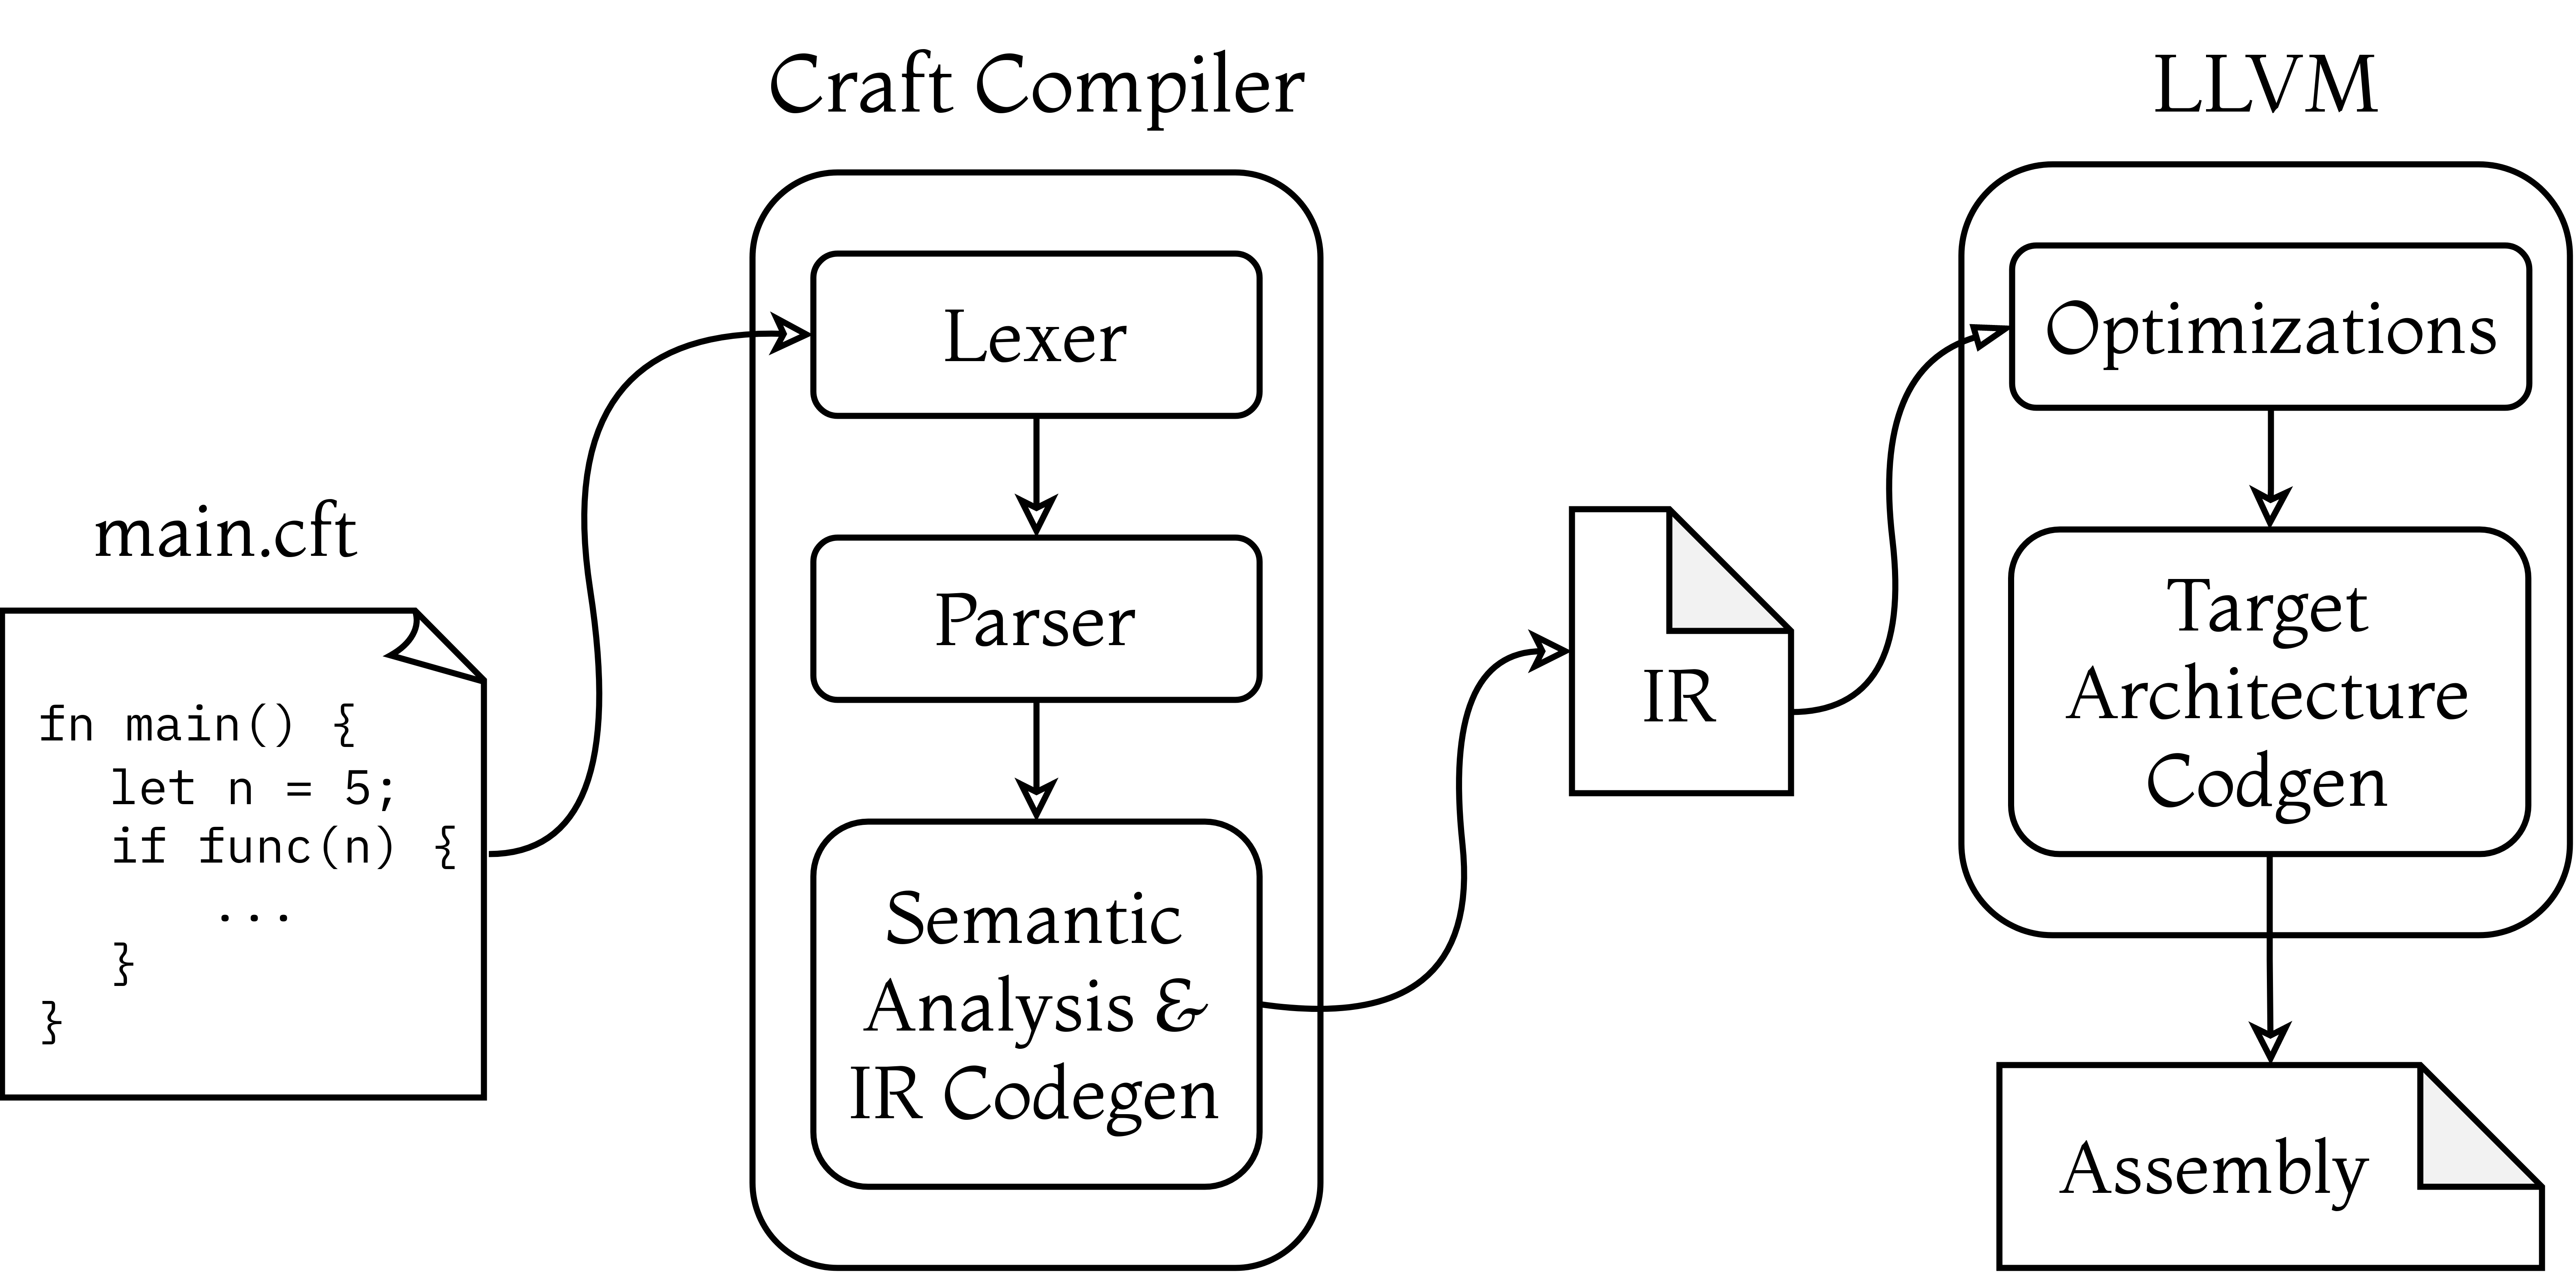
\includegraphics[width=\linewidth]{arch}
\caption{Diagram showing the compilation workflow of a Craft program}
\end{figure}


\section{Results}
\section{Conclusions}

\begin{thebibliography}{11}
\bibitem{latex}
http://en.wikibooks.org/wiki/LaTeX

\bibitem{2}
Referència 2

\bibitem{3}
Etc.

\end{thebibliography}

\appendix

\section*{Apèndix}

\setcounter{section}{1}

\subsection{Secció d'Apèndix}
.... ... ..... ... ..... ... ... ..... .... .

\subsection{Secció d'Apèndix}
.... ... ..... ... ..... ... ... ..... .... .

\end{document}
